
\subsection{Histogram computation}
\label{sec:histogram}

A histogram succinctly and meaningfully summarizes the data, thus histogram computation is a very
common analysis task. In this section, we study bit streams that aim to reproduce the most accurate
histogram possible at any bit rate. It is necessary to first define a criteria to compare two
histograms. We choose to use the popular Earth mover's distance as the distance metric for
histograms [CITE]. With the error metric defined, Algorithm [REF] gives us a
\emph{histogram-optimized} stream, given an input data set. To understand the characteristics of an
\emph{histogram-optimized} stream that make it suitable for histogram computation, we compare it
with the \emph{rmse-optimized} stream for the same data set. We also include their corresponding
data-independent analouges, namely \emph{histogram signature} and \emph{by wavelet norm} (the
concept of a signature is defined in Section [REF]). Figures \ref{fig:histogram-stream-comparison}
are plots of the EMD errors for these streams on four data sets.

\begin{figure}[h]
	\centering
	\subcaptionbox{\emph{boiler}, 64 bins}
	{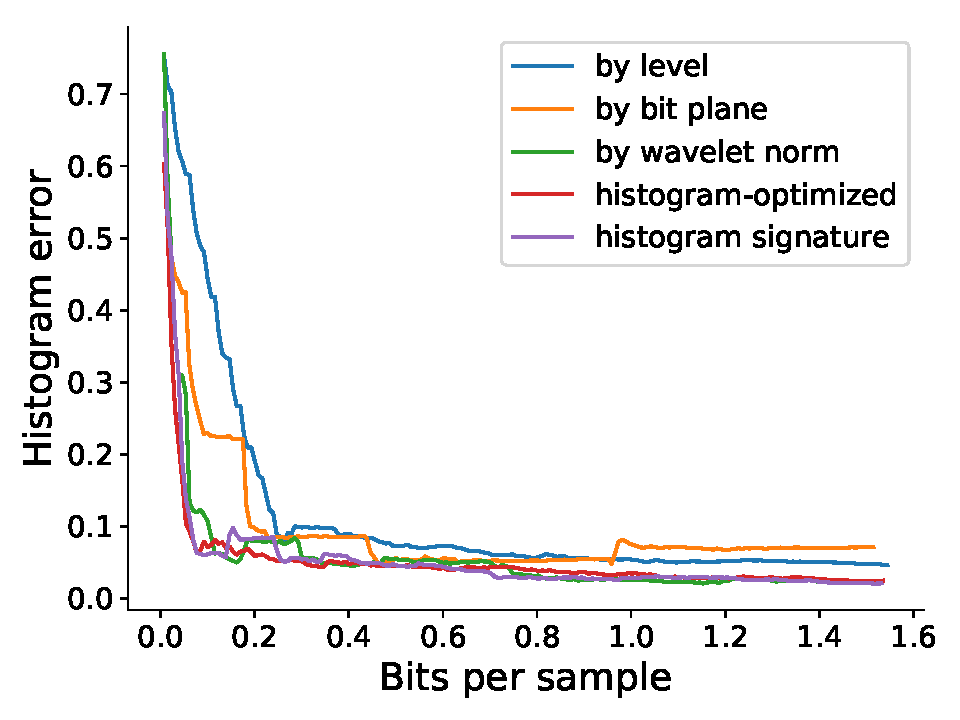
\includegraphics[width=0.48\linewidth]{img/histogram/64bins/histogram-optimized-boiler.pdf}}
	\subcaptionbox{\emph{diffusivity}, 64 bins}
	{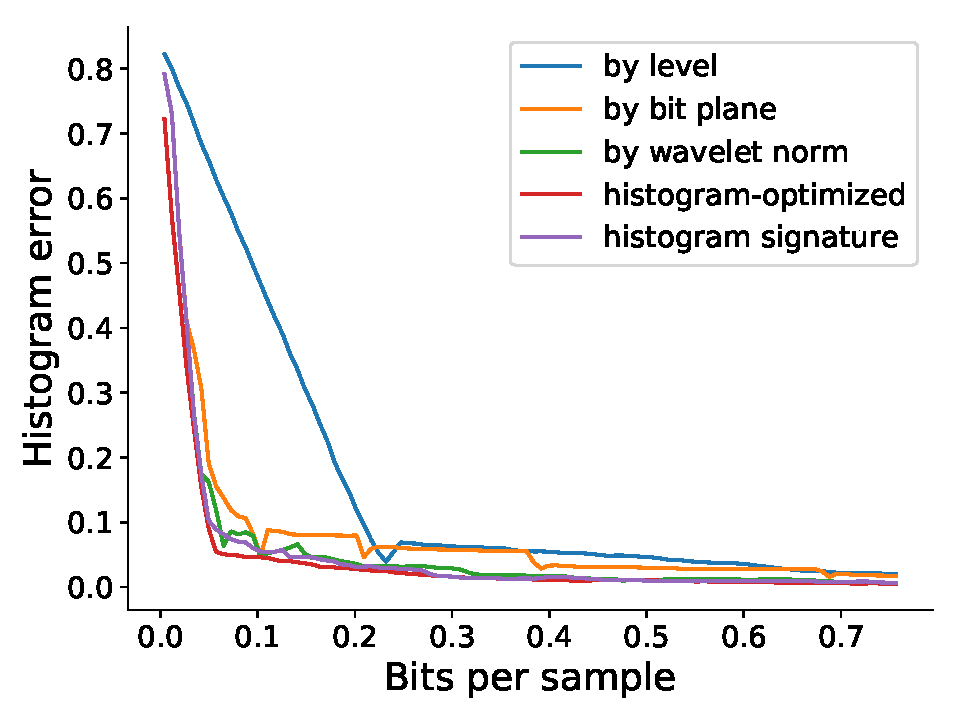
\includegraphics[width=0.48\linewidth]{img/histogram/64bins/histogram-optimized-diffusivity.pdf}}
	\subcaptionbox{\emph{euler}, 64 bins}
	{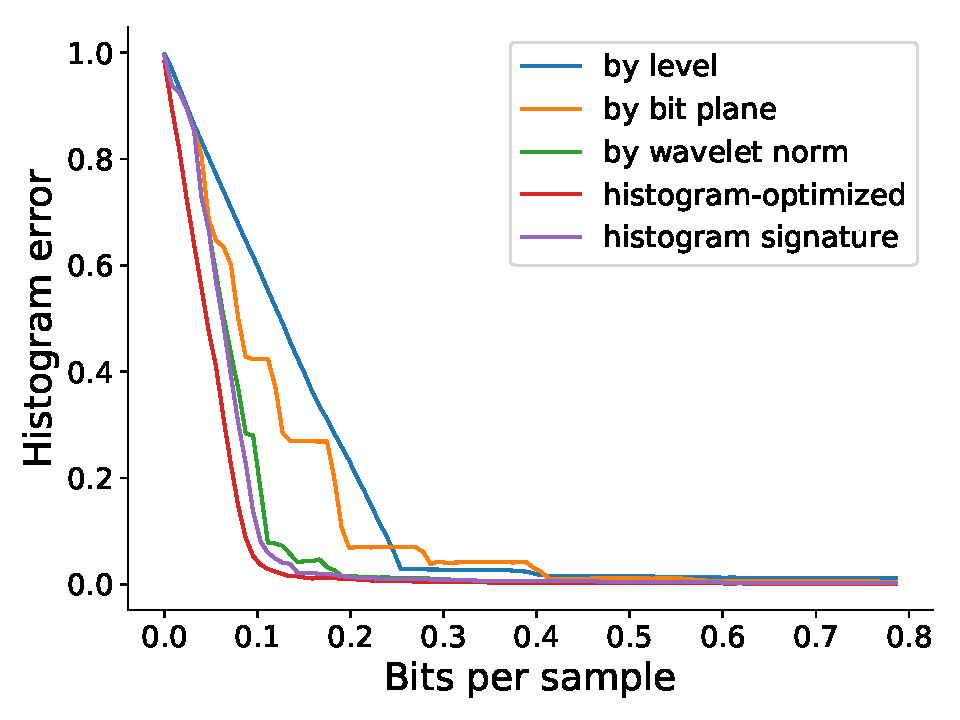
\includegraphics[width=0.48\linewidth]{img/histogram/64bins/histogram-optimized-euler.pdf}}
	\subcaptionbox{\emph{pressure}, 64 bins}
	{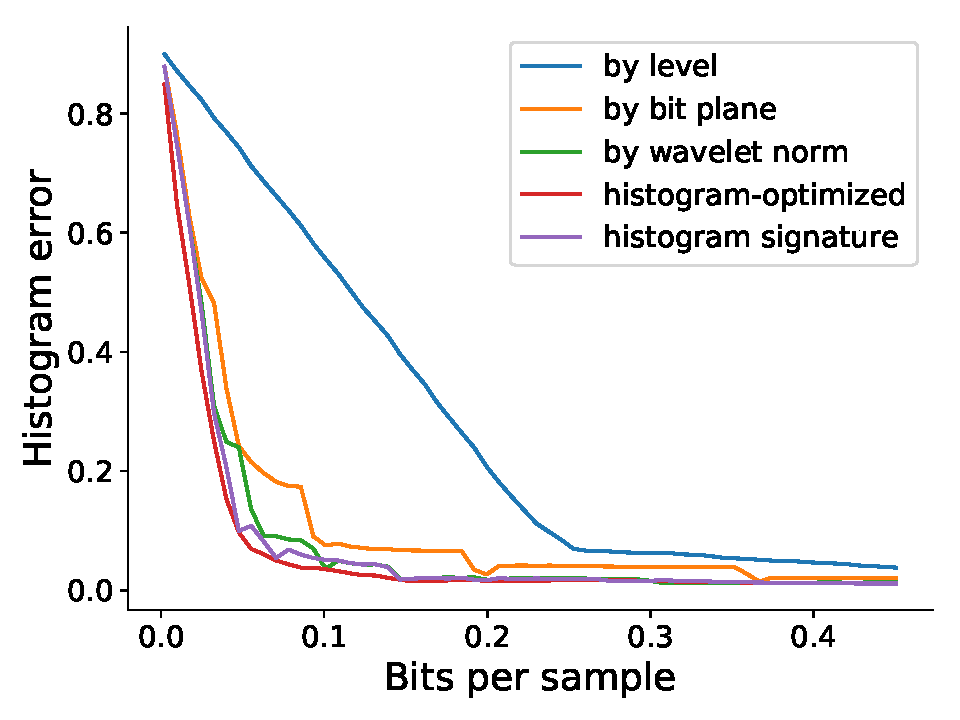
\includegraphics[width=0.48\linewidth]{img/histogram/64bins/histogram-optimized-pressure.pdf}}
	% \subcaptionbox{\emph{turbulence}, 64 bins}
	% {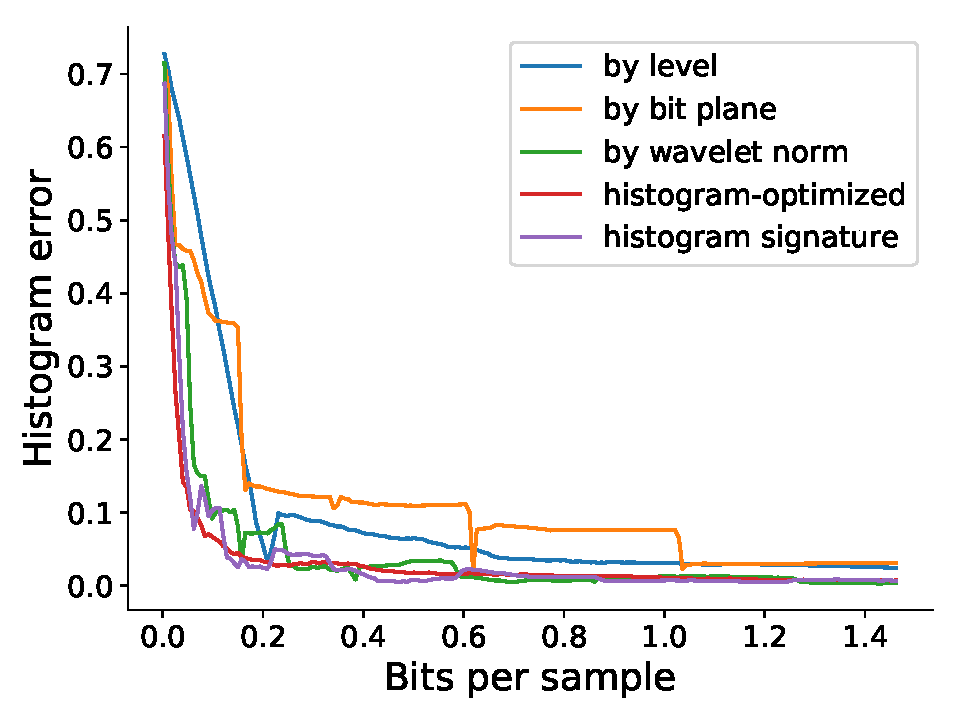
\includegraphics[width=0.48\linewidth]{img/histogram/64bins/histogram-optimized-turbulence.pdf}}
	% \subcaptionbox{\emph{velocityz}, 64 bins}
	% {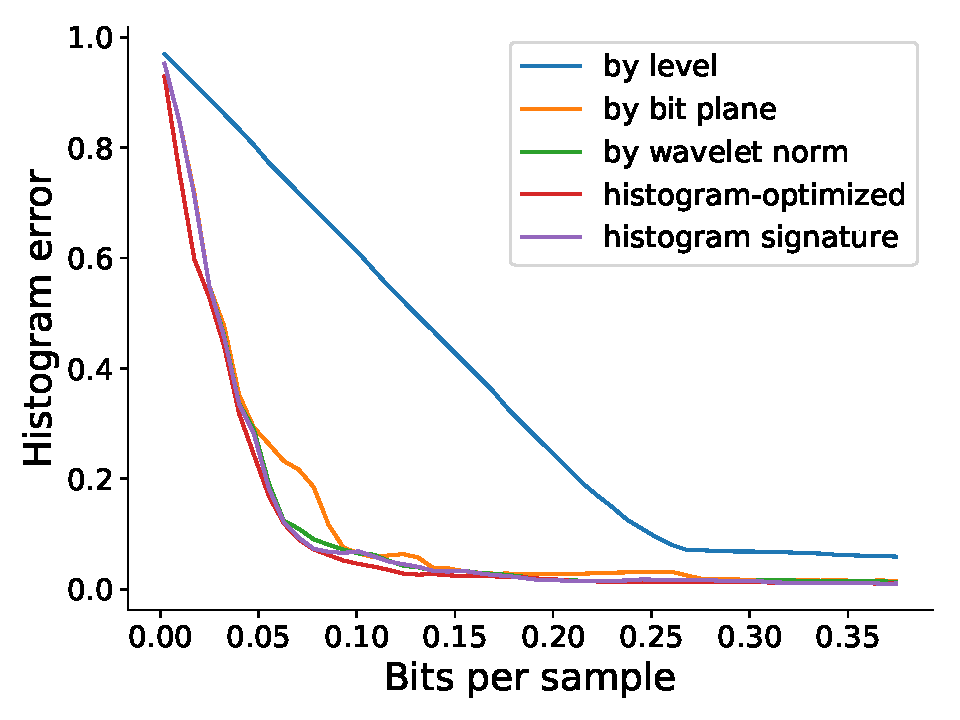
\includegraphics[width=0.48\linewidth]{img/histogram/64bins/histogram-optimized-velocityz.pdf}}
	\caption{Histogram error comparison among four streams \emph{histogram-optimized},
	\emph{rmse-optimized}, \emph{by wavelet norm}, and \emph{histogram signature}, without the leading
	zero bits. The plots are truncated to make the differences large enough for visual inspection, and
	truncation points are chosen so that the best among the reconstructed histograms is visually the
	same as the groundtruth histogram. }
	\label{fig:histogram-stream-comparison}
\end{figure}

First, compared to \emph{rmse-optimized}, the \emph{histogram-optimized} stream produces
consistently better histograms. Second, between the two data-independent streams, \emph{histogram
signature} outperforms \emph{by wavelet norm}. To better understand how the Earth mover's distance
translates to visual differences, we visualize the histograms produced by the different streams, at
low bit rates, in Figure \ref{fig:histogram-comparison-low-bit-rate}. These plots confirm our
observations.
\emph{histogram-optimized} and \emph{histogram signature}
outperform \emph{rmse-optimized} and \emph{by wavelet norm} respectively. For example, Figure
\ref{fig:histogram-comparison-low-bit-rate-slz} shows the four reconstructed histograms at 0.1 bits
per sample, with leading zero bits removed, for the diffusivity data set.

\begin{figure}[h]
	\centering
	\subcaptionbox{\emph{boiler}, 0.24 bps}
	{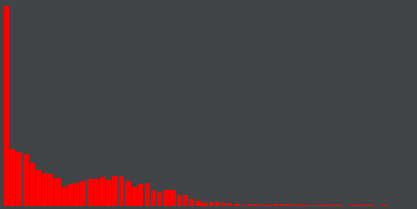
\includegraphics[width=0.32\linewidth]{img/histogram/histogram-renderings/histogram-boiler-by-wavelet-norm.png}}
	{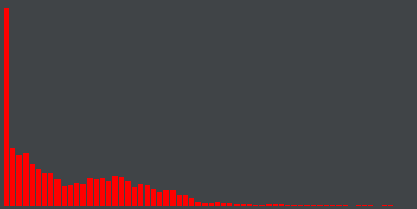
\includegraphics[width=0.32\linewidth]{img/histogram/histogram-renderings/histogram-boiler-signature.png}}
	{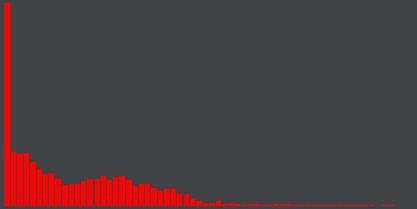
\includegraphics[width=0.32\linewidth]{img/histogram/histogram-renderings/histogram-boiler-groundtruth.png}}
	\subcaptionbox{\emph{diffusivity}, 0.75 bins}
	{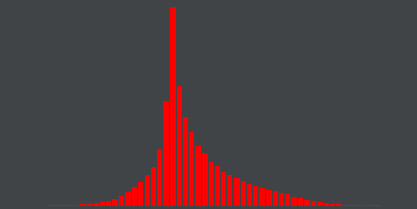
\includegraphics[width=0.32\linewidth]{img/histogram/histogram-renderings/histogram-diffusivity-by-wavelet-norm.png}}
	{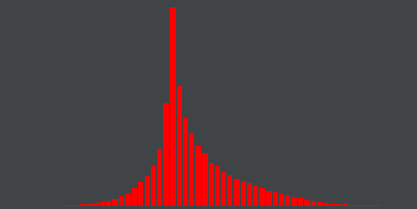
\includegraphics[width=0.32\linewidth]{img/histogram/histogram-renderings/histogram-diffusivity-signature.png}}
	{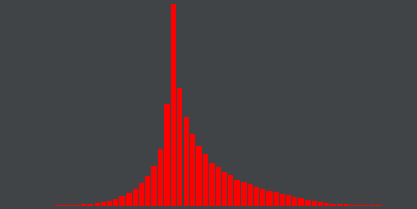
\includegraphics[width=0.32\linewidth]{img/histogram/histogram-renderings/histogram-diffusivity-groundtruth.png}}
	\subcaptionbox{\emph{euler}, 0.28 bins}
	{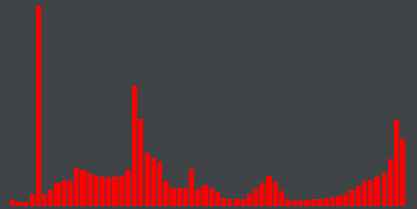
\includegraphics[width=0.32\linewidth]{img/histogram/histogram-renderings/histogram-euler-by-wavelet-norm.png}}
	{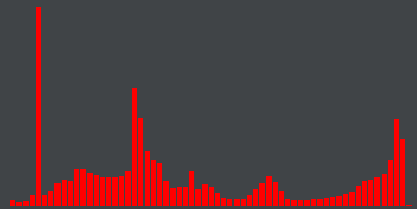
\includegraphics[width=0.32\linewidth]{img/histogram/histogram-renderings/histogram-euler-signature.png}}
	{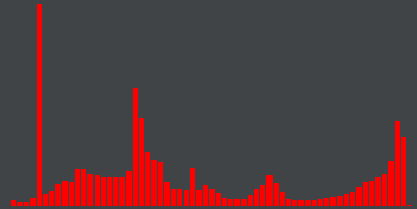
\includegraphics[width=0.32\linewidth]{img/histogram/histogram-renderings/histogram-euler-groundtruth.png}}
	\subcaptionbox{\emph{pressure}, 0.64 bps}
	{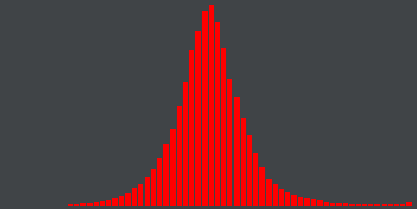
\includegraphics[width=0.32\linewidth]{img/histogram/histogram-renderings/histogram-pressure-by-wavelet-norm.png}}
	{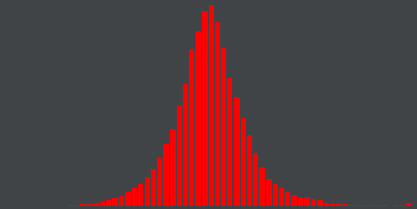
\includegraphics[width=0.32\linewidth]{img/histogram/histogram-renderings/histogram-pressure-signature.png}}
	{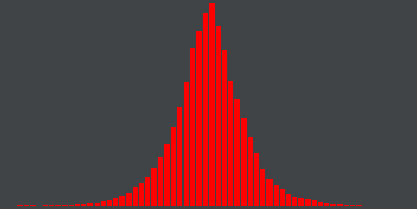
\includegraphics[width=0.32\linewidth]{img/histogram/histogram-renderings/histogram-pressure-groundtruth.png}}
	% \subcaptionbox{\emph{turbulence}, 0.75 bps}
	% {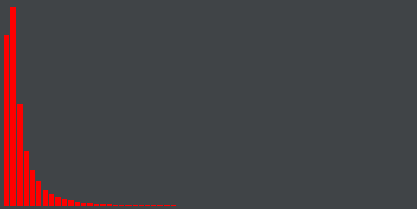
\includegraphics[width=0.32\linewidth]{img/histogram/histogram-renderings/histogram-turbulence-by-wavelet-norm.png}}
	% {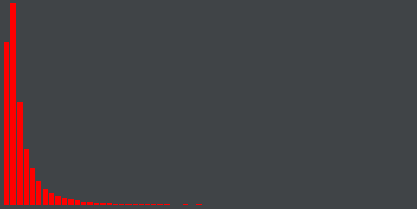
\includegraphics[width=0.32\linewidth]{img/histogram/histogram-renderings/histogram-turbulence-signature.png}}
	% {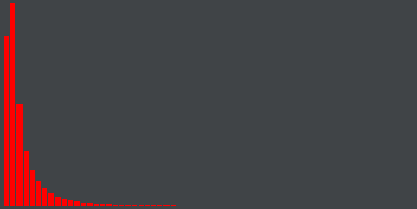
\includegraphics[width=0.32\linewidth]{img/histogram/histogram-renderings/histogram-turbulence-groundtruth.png}}
	% \subcaptionbox{\emph{velocityz}, 1.19 bps}
	% {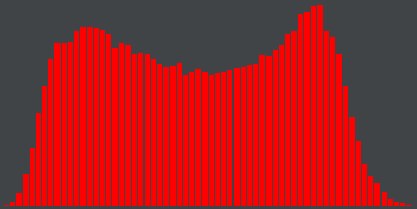
\includegraphics[width=0.32\linewidth]{img/histogram/histogram-renderings/histogram-velocityz-by-wavelet-norm.png}}
	% {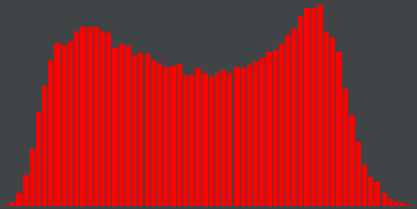
\includegraphics[width=0.32\linewidth]{img/histogram/histogram-renderings/histogram-velocityz-signature.png}}
	% {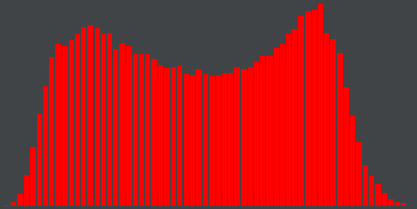
\includegraphics[width=0.32\linewidth]{img/histogram/histogram-renderings/histogram-velocityz-groundtruth.png}}
	\caption{Histogram error comparison among four streams \emph{histogram-optimized},
	\emph{rmse-optimized}, \emph{by wavelet norm}, and \emph{histogram signature}, without the leading
	zero bits. The plots are truncated to make the differences large enough for visual inspection, and
	truncation points are chosen so that the best among the reconstructed histograms is visually the
	same as the groundtruth histogram. }
	\label{fig:histogram-stream-comparison}
\end{figure}

% \begin{figure}
% 	\centering
% 	\subcaptionbox{\emph{histogram-optimized}}
% 	{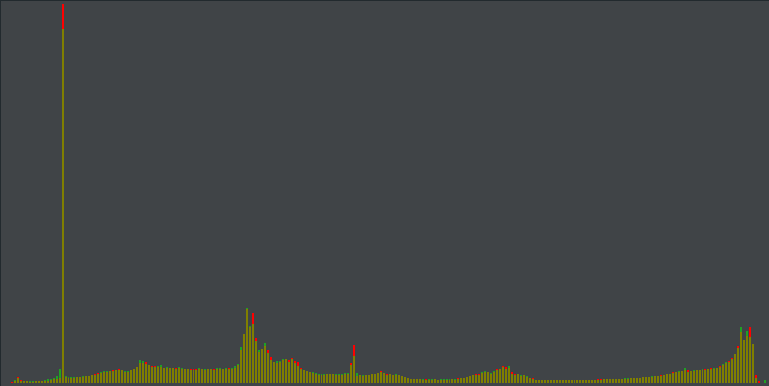
\includegraphics[width=0.48\linewidth]{img/histogram/histogram-signature.png}}
% 	\subcaptionbox{\emph{rmse-optimized}}
% 	{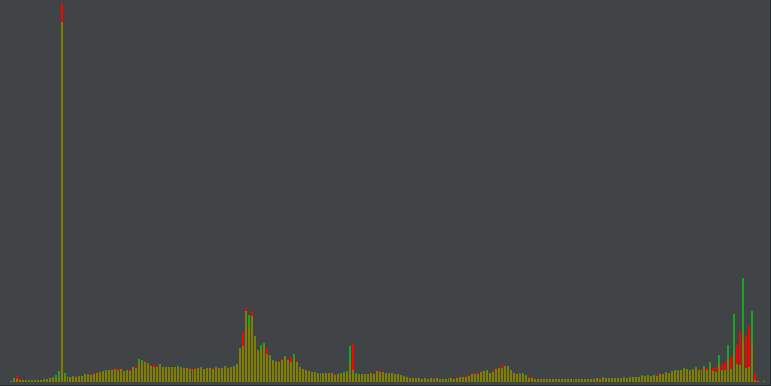
\includegraphics[width=0.48\linewidth]{img/histogram/histogram-by-wavelet-norm.png}}
% 	\caption{euler's histograms at 0.18 bps. The groundtruth histogram is rendered in red, while the
% 	reconstructed histogram is rendered in green. The dark yellow regions are where the two overlap.}
% 	\label{fig:histogram-comparison-low-bit-rate-slz}
% \end{figure}

The main difference between the \emph{histogram-optimized} and the \emph{rmse-optimized} streams is
that \emph{histogram-optimized} favors low-ordered bits of coarse-level coefficients, while,
\emph{rmse-optimized} relatively favors high-ordered bits of fine-level coefficients. This is
evident in Figure \ref{fig:histogram-signature-comparison} (b and d): for
\emph{histogram-optimized}, the bright blue cells extend more toward the right (lower-ordered bit
planes) and less toward the bottom (finer resolution levels). The histogram experiments in this
Section are performed with 256 bins, but this fact holds for a wide range of number of bins. Figures
\ref{fig:histogram-signature-comparison} (a, b, c) show that varying the number of bins from 128 to
512 only affects the relative ordering among the low-ordered bits on very fine resolution levels
(the dark blue cells at the bottom right of the signature). These are bits that come at the end of a
stream, and thus matter little to the data quality. 

The streams in Figure \ref{fig:histogram-comparison-low-bit-rate} (b, d, f, h) are truncated where
the EMD errors of the \emph{histogram-optimized} streams are negligible, suggesting that it is often
possible to achieve near lossless histograms with just 1 bit per sample. The boiler data set is a
peculiar case, where the \emph{histogram-optimized} stream outperforms the rest of the streams by a
large margin in the second half of the bit rate range. Looking at the precision maps (defined in
Section [REF]) for the \emph{histogram-optimized} stream, as well as its reconstructed histogram
(Figure \ref{fig:precision-map-histogram}, (a)), we see that the bit distribution is heavily
concentrated in regions corresponding to one particular histogram bin that contains vastly more
samples than other bins do. This situtation happens when there are many samples having essentially
the same value but they are distributed irregularly in space (otherwise they would form constant
regions which would be captured very well with just a few precision bits of wavelet coefficients --
this is the case for the flame data set). In this case a stream needs to be more spatially adaptive
to resolve well the histogram bin with the most samples, and among the tested streams, only
\emph{histogram-optimized} is spatially adaptive to EMD (\emph{rmse-optimized} is spatially
adaptive, but to RMSE, and the other two streams are data-independent).

% \begin{figure}[h]
% 	\centering
% 	\subcaptionbox{}
% 	{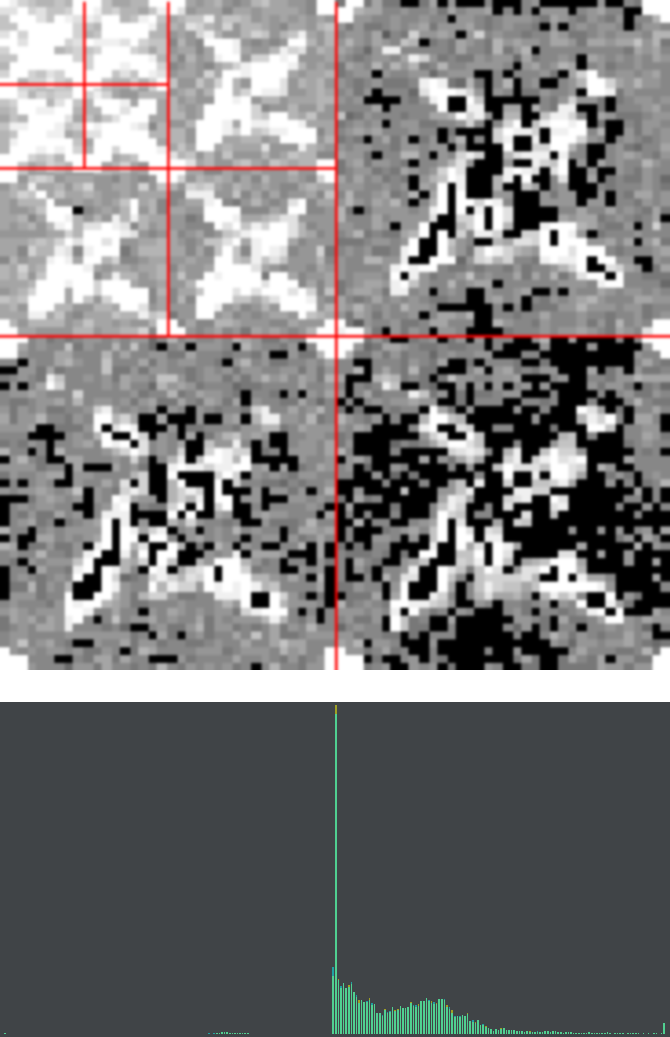
\includegraphics[width=0.24\linewidth]{img/histogram/boiler/prec-histogram_resize-vert.png}}
% 	\subcaptionbox{}
% 	{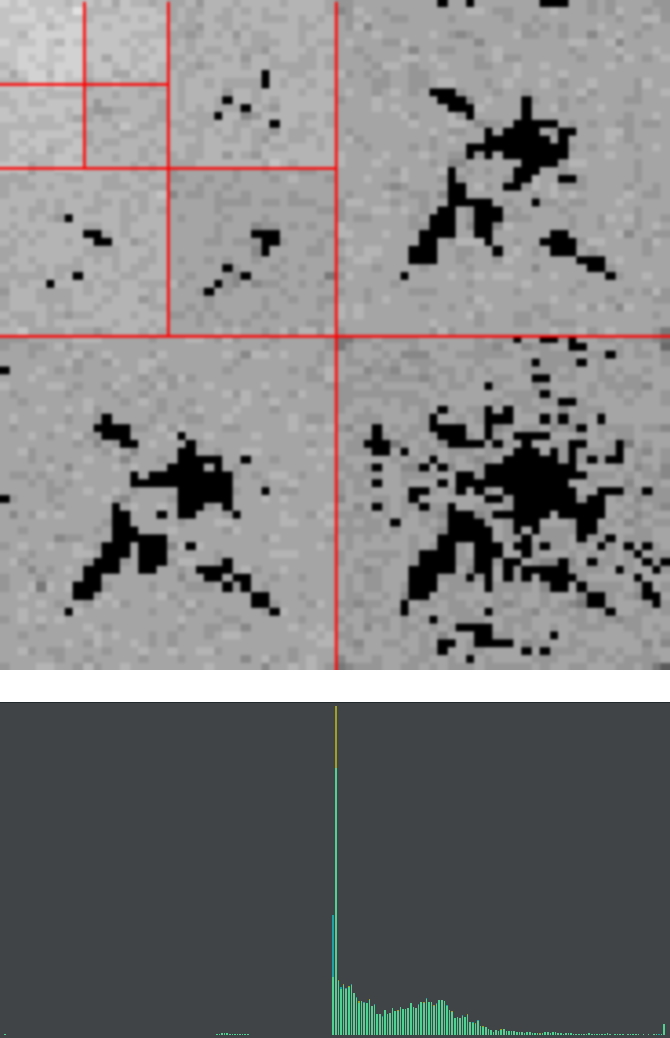
\includegraphics[width=0.24\linewidth]{img/histogram/boiler/prec-rmse_resize-vert.png}}
% 	\subcaptionbox{}
% 	{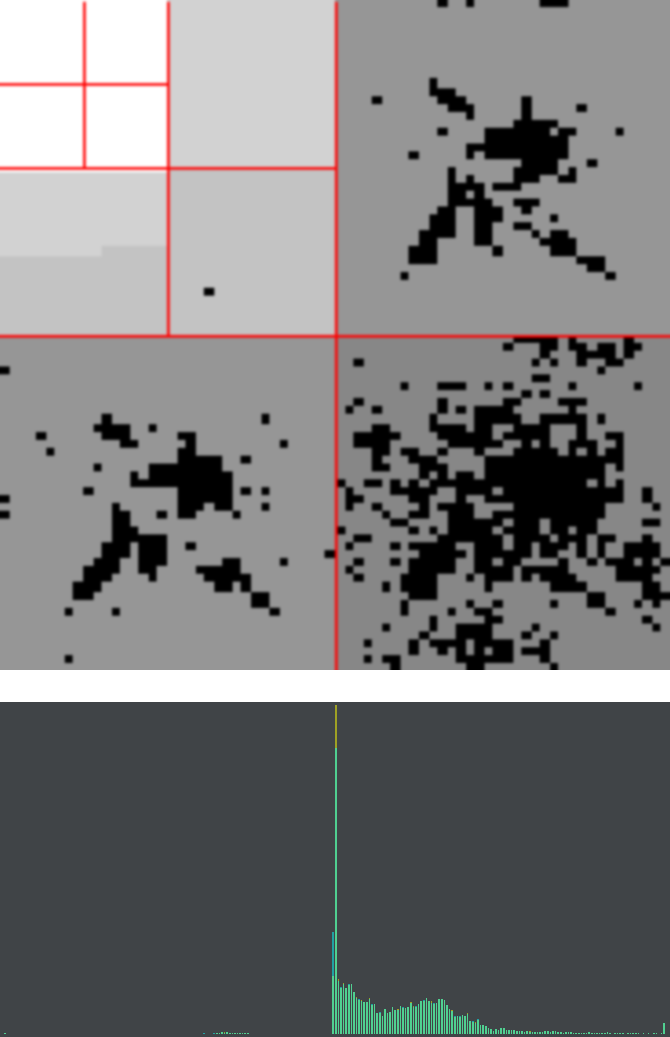
\includegraphics[width=0.24\linewidth]{img/histogram/boiler/prec-signature_resize-vert.png}}
% 	\subcaptionbox{}
% 	{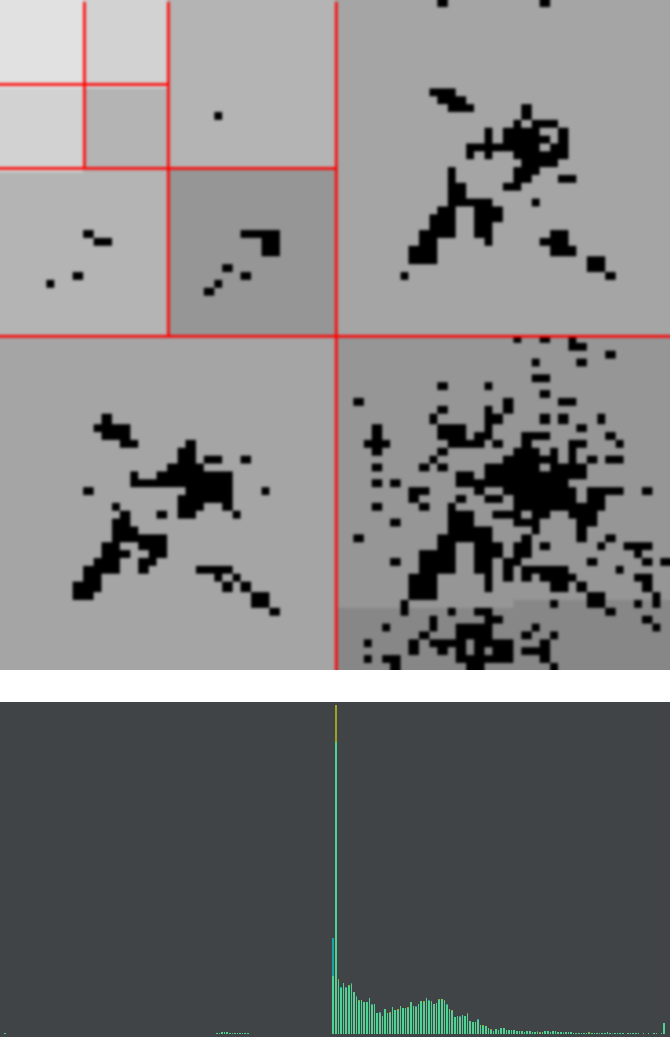
\includegraphics[width=0.24\linewidth]{img/histogram/boiler/prec-wavenorm_resize-vert.png}}
% 	\caption{(top) Precision distribution of wavelet coefficients, and (bottom) reconstructed
% 	histograms, for \emph{histogram-optimized}, \emph{rmse-optimized}, \emph{by wavelet norm}, and
% 	\emph{histogram signature} streams, at 6.47 bits per sample, without leading zero bits.}
% 	\label{fig:precision-map-histogram}
% \end{figure}

TODO: discuss the case of not using compression, where the signature plays a more important role.

In this section we have shown that histogram computation requires a different ordering of bits than
reconstructing the function itself. We have also proposed a practical heuristic, based on stream
signatures, to capture the main characteristics of this ordering. In practice, the histogram
signature can be pre-computed once and stored on disk. A signature's size is negligible (170
integers in 2D and 374 integers in 3D in the case of four wavelet levels in each dimension), and can
also be further compressed. Therefore it can be transmitted first, and the receiver of the data can
ultilize the signature to smartly query the bits so as to reconstruct the data's histogram with as
few bits as possible.
%%% Local Variables:
%%% mode: latex
%%% TeX-master: "template"
%%% End:
